\documentclass{article}

%%%% Patch to make lineno work nicely with amsmath
% https://tex.stackexchange.com/a/461192
\usepackage{lineno}
\usepackage{amsmath}  %% <- after lineno
\usepackage{etoolbox} %% <- for \cspreto, \csappto
%% Patch 'normal' math environments:
\newcommand*\linenomathpatch[1]{%
  \cspreto{#1}{\linenomath}%
  \cspreto{#1*}{\linenomath}%
  \csappto{end#1}{\endlinenomath}%
  \csappto{end#1*}{\endlinenomath}%
}
\linenomathpatch{equation}
\linenomathpatch{gather}
\linenomathpatch{multline}
\linenomathpatch{align}
\linenomathpatch{alignat}
\linenomathpatch{flalign}
\linenumbers%
%%%% end patching

\usepackage{amsfonts}
\usepackage{amssymb}
\usepackage{amsthm}
\usepackage{graphicx}
\usepackage[hidelinks]{hyperref}
\usepackage[inline]{showlabels}
\renewcommand{\showlabelfont}{\tiny\sffamily}

\newtheorem{lemma}{Lemma}
\newtheorem{prop}{Proposition}
\newtheorem{thm}{Theorem}
\newtheorem{prob}{Problem}
\newtheorem{defn}{Definition}
\newtheorem{obs}{Observation}
\newtheorem{alg}{Algorithm}

\newcommand{\median}{\operatorname{median}}

% http://bytesizebio.net/2013/03/11/adding-supplementary-tables-and-figures-in-latex/
\newcommand{\beginsupplement}{%
        \setcounter{table}{0}
        \renewcommand{\thetable}{S\arabic{table}}%
        \setcounter{figure}{0}
        \renewcommand{\thefigure}{S\arabic{figure}}%
     }

\hyphenation{Ge-nome Ge-nomes hyper-mut-ation through-put}

% template follows "Ten simple rules for structuring papers" http://dx.doi.org/10.1371/journal.pcbi.1005619

\title{Focus your paper on a central contribution, and communicate that in the title}
\author{You}

\begin{document}
\maketitle

\begin{abstract}
% The one question is:
% Here we... (describe approach)
% What we found
% How it matters
\end{abstract}


\section*{Introduction}
% At least one paragraph for each of the following prompts.

% Describe the big problem in science we are approaching here.

% What does the field know about this problem?

% What is the remaining gap?

% In this paper, we... (Describe approach)

% We find that...


Hooray for Joe~\cite{Felsenstein1981-zs}.

% NOTE: here I'm writing a results-first paper. A methods-first paper should
% still have a Methods overview before really getting into the details.
\section*{Results}

\subsection*{Methods overview}
% In order to [insert research question statement] we developed a method...
% Here we give a brief overview of how this method works; full details can be found in the Methods section.

\begin{figure}[h]
\centering
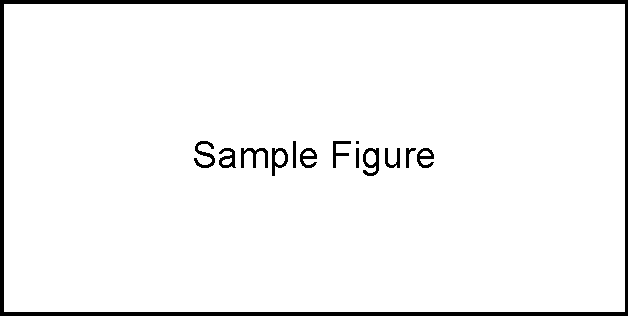
\includegraphics[width=0.35\textwidth]{figures/sample-figure.pdf}
\caption{\
Sample figure demonstrating the build process.
}%
\label{fig:sample}
\end{figure}


% Now there should be a succession of section headings that are findings, such as
% \subsection*{7 is bigger than 6 but less than 8}


\section*{Discussion}

% ** Important **: The discussion is your final chance to make the case for your research. Here you have the opportunity to carefully compare what you have done to what was already known.

% What we found (brief summary)

% Our work in the context of other research (more in depth)

% Limitations

% Why science is better now, and prospects for future work


\section*{Materials and methods}

\subsection*{Data}

% Then whatever methods details you have.


\bibliographystyle{plainurl}
\bibliography{main}


% \clearpage
% \section*{Supplementary Materials}
% \beginsupplement
% Supplementary text and figures here.


\end{document}
